\begin{blocksection}
% \question Mario needs to jump over a series of Piranha plants, represented as a
% string of P's and \lstinline$P$'s. Mario only moves forward and can
% either \emph{step} (move forward one space) or \emph{jump} (move forward two
% spaces) from each position. How many different ways can Mario traverse a level
% without stepping or jumping into a Piranha plant? Assume that every level begins
% with a \lstinline$-$ (where Mario starts) and ends with a \lstinline$-$ (where
% Mario must end up).

% \begin{lstlisting}
% def mario_number(level):
%     """
%     >>> mario_number('-P-P-')
%     1
%     >>> mario_number('-P-P--')
%     1
%     >>> mario_number('--P-P-')
%     1
%     >>> mario_number('---P-P-')
%     2
%     >>> mario_number('-P-PP-')
%     0
%     >>> mario_number('----')
%     3
%     >>> mario_number('----P----')
%     9
%     >>> mario_number('---P----P-P---P--P-P----P-----P-')
%     180
%     """
% \end{lstlisting}

% \begin{solution}[1in]
% \begin{lstlisting}
%     if len(level) == 0 or level[0] == 'P':
%         return 0
%     elif len(level) <= 2:
%         return 1
%     else:
%         return mario_number(level[1:]) + mario_number(level[2:])
% \end{lstlisting}
% \end{solution}

\question Mario needs to get from one end of a level to the other, but there are deadly Piranha plants in his way! Mario only moves forward and can
either \emph{step} (move forward one space) or \emph{jump} (move forward two
spaces) from each position. A level is represented as a series of ones and zeros, with zeros denoting the location of Piranha plants. Mario can step on ones but not on zeros.  How many different ways can Mario traverse a level
without stepping or jumping into a Piranha plant? Assume that every level begins
with a 1 (where Mario starts) and ends with a 1 (where
Mario must end up).

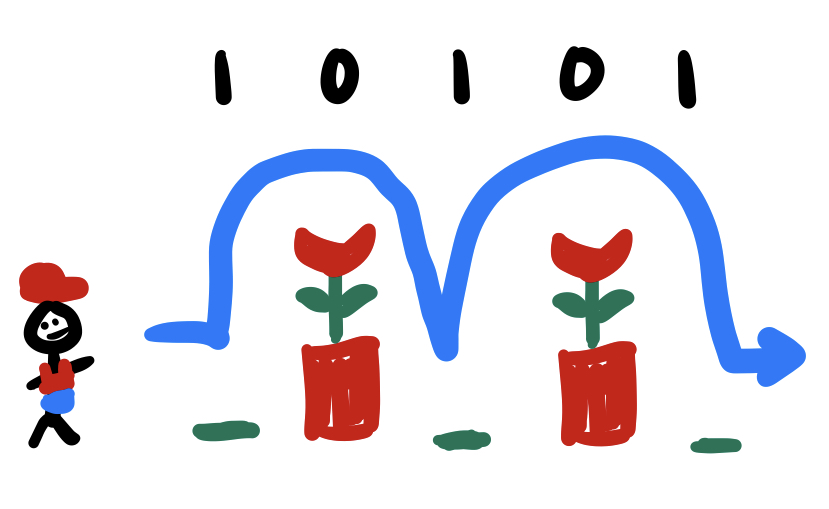
\includegraphics[scale=0.2]{mario_number_10101.jpg}
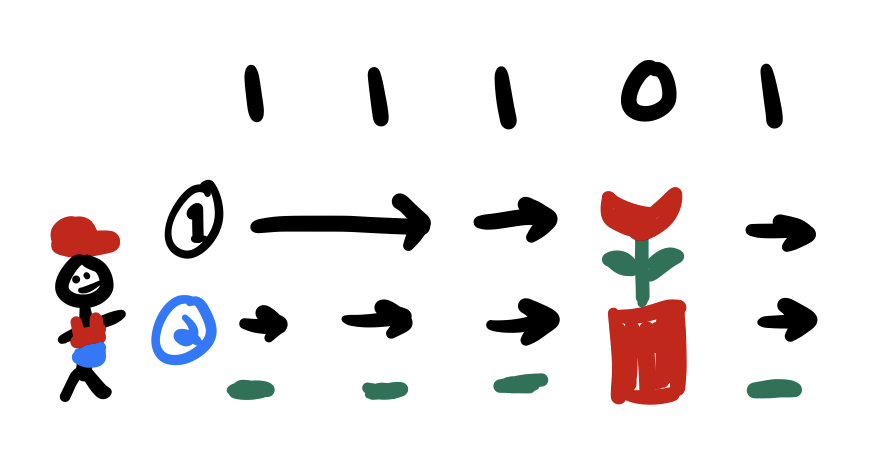
\includegraphics[scale=0.2]{mario_number_11101.jpg}


\textit{Hint: Does it matter whether Mario goes from left to right or right to left? Which
one is easier to check?}
\end{blocksection}
\begin{blocksection}
\begin{lstlisting}
def mario_number(level):
    """
    >>> mario_number(10101)
    1
    >>> mario_number(11101)
    2
    >>> mario_number(100101)
    0
    """
    if _______________________:

        ______________________

    elif _____________________:

        ______________________

    else:

        ___________________________________________________
\end{lstlisting}
\end{blocksection}

\begin{solution}
\begin{blocksection}
\begin{lstlisting}
def mario_number(level):
    if level == 1:
        return 1
    elif level % 10 == 0:
        return 0
    else:
        return mario_number(level // 10) + mario_number((level // 10) // 10)
\end{lstlisting}
You can think about this tree recursion problem as testing out all of the possible ways Mario can traverse the level, and adding 1 every time you find a possible traversal.

Here it doesn't matter whether Mario goes left to right or right to left; either way we'll end up with the same number of ways to traverse the \lstinline{level}. In that case, we can simply choose for Mario to start from the right, and then we can process the level like we process other numbers in digit-parsing related questions by using floor division (\lstinline{//}) and modulo (\lstinline{%})

At each point in time, Mario can either step or jump. We use a single floor division (\lstinline{//}) of \lstinline{level} by 10 to represent taking one step (if we took a step, then the entire \lstinline{level} would be left except for the last number), while two floor divisions by 10 (or equivalently one floor division by 100) corresponds to a jump at this point in the \lstinline{level} (if we took a jump, then the entire \lstinline{level} would be left except for the last two numbers).

To think of the base cases, you can consider the two ways that Mario ends his journey. The first, corresponding to \lstinline{level == 1}, means that Mario has successfully reached the end of the level. You can \lstinline{return 1} here, because this means you've found one additional path to the end. The second, corresponding to \lstinline{level % 10 == 0}, means that Mario has landed on a Piranha plant. This returns 0 because it's a failed traversal of the \lstinline{level}, so you don't want to add anything to your result.

In tree recursion, you need to find a way to combine separate recursive calls. In this case, because \lstinline{mario_number} returns an integer and the base cases are integers and you're trying to count the total number of ways of traversal, it makes sense to add your recursive calls.

\end{blocksection}
\end{solution}

\begin{questionmeta}
\textbf{Teaching Tips}
\begin{itemize}
    \item Some leading questions:
    \begin{itemize}
        \item What are our base cases? (When do we know we've reached the end of the level? When do we know that we've failed?)
        \item Is there any difference between going left to right or right to left in terms of the number of ways to traverse the level?
        \item What are our two options at each step?
        \item What do those look like in a recursive call?
        \item How should we combine our recursive calls? (and, or, addition, etc.)
    \end{itemize}
    \item Try leaning into the narrative of the question! It's fun and can help rephrase recursive calls ``in plain english''
          I also like drawing the problem out along with the doctests to visualize the different steps Mario can take :D !
    \item It's very useful to draw a tree diagram! Each function call has one branch for stepping once and another branch for stepping twice. Each branch then has 2 branches of their own (until a base case is reached).
    \item Teach students that recursive calls can be treated as numbers using the recursive leap of faith, so combining the two recursive call branches with addition is really just adding two numbers.
\end{itemize}
\end{questionmeta}
